%\documentclass[10pt]{article}\usepackage[correction,nu]{esial}
\documentclass[10pt]{article}\usepackage[nu]{esial}
\usepackage{amstext,amsmath,amsfonts}
\TOP\unA
\newcommand{\WP}[1]{\textbf{WP}($#1$)}

\usepackage{amsthm,pifont,textcomp}
\usepackage{amsmath,amssymb}

\usepackage[utf8]{inputenc}
\graphicspath{{fig/}}

\begin{document}
\title{Examen du 16/06/2011 (1h)}
\fvset{fontsize=\footnotesize}
\maketitle\vspace{-\baselineskip}

\begin{center}
  \textbf{\large Documents interdits, à l'exception d'une feuille A4 à rendre
    avec votre copie.}

  \noindent\textit{La notation tiendra compte de la présentation et de la
    clarté de la rédaction.}

  \textit{Le barême, approximatif, est donné sur 10 points puisque l'épreuve
    dure 1h ($\frac{10}{20}=0,5=\frac{1h}{2h}$).}
\end{center}\vspace{-\baselineskip}
%\smallskip


\bigskip\QuestionCours~(2pt)

\Question(1pt) À quelles classes de complexité (en notation
$\Theta$) appartiennent les algorithmes 1 et 2 suivants?

\medskip\noindent\begin{minipage}{.45\linewidth}
  \begin{Verbatim}[label=algorithme 1]
pour i = 1 à n faire
  pour j = 1 à n faire
     x += 3    
  \end{Verbatim}
\end{minipage}\hfill\begin{minipage}{.45\linewidth}
  \begin{Verbatim}[label=algorithme 2]
pour i = 1 à n faire
  pour j = 1 à n faire
    x += 3
pour i = 1 à n faire
  y = x + 5
  \end{Verbatim}
\end{minipage}

\Question(1pt) Définissez les types de récursivité suivants: terminale,
générative, mutuelle (ou croisée) et structurelle.

\medskip\Exercice\textbf{Code récursif mystère} (5pts). 
 %
Considérez le code mystère suivant. 

\noindent\begin{minipage}{.65\linewidth}

\Question(\textonehalf pt) Explicitez les appels récursifs effectués pour 
\texttt{puzzle(25,4)}. 

\Question(1pt) Calculez le résultat de la fonction puzzle pour les valeurs
suivantes. 
(10,1) (10,2) (10,3) (10,4) (10,6) (10,8) (10,10)\\
Que semble calculer \texttt{puzzle()}? 

\end{minipage}\hfill
\begin{minipage}{.33\linewidth}
\begin{Verbatim}[numbers=right]
public int puzzle(int i, int j) {
  if (i == 1)     
    return j;
  if (i % 2 == 1)
    return j+puzzle(i/2,j*2);
  else 
    return   puzzle(i/2,j*2);
}
\end{Verbatim}
\end{minipage}

\Question(\textonehalf pt)  Montrez la terminaison de cet algorithme. 

\Question(\textonehalf pt) Quelle est la complexité algorithmique de \texttt{puzzle} (en
nombre d'appels récursifs)? 

\Question(\textonehalf pt) Est-il possible de dérécursiver directement cette
fonction ? Pourquoi ? 

\Question(2pts) Dérécursivez cette fonction en appliquant les méthodes vues en cours
(en une ou plusieurs étapes). Explicitez ce que vous faites et
pourquoi. 


\medskip
\Exercice\textbf{Identification d'algorithmes de tri} (d'après Aldo Cortesi --
3pt).

Les schémas suivants montrent le fonctionnement de divers algorithmes de
tris. Chaque trait grisé indique une valeur, et l'axe des abscisses montre le
temps qui passe tandis que l'axe des ordonnées montre la position de chaque
valeur (=trait) dans les différentes cases du tableau. La case n°1 est en haut,
et la case n°20 est en bas, et une couleur plus claire signifie une valeur plus
petite. Quand deux traits se croisent, c'est que l'algorithme a inversé les
deux valeurs à cet instant.

\Question Identifiez le comportement des algorithmes suivants: tri à bulle, tri
par insertion, tri par sélection, shell sort, quick sort. Argumentez vos
réponses. 

\bigskip

\noindent\hspace{-4em}\hbox to 1.2\linewidth{\hfill\begin{minipage}{.35\linewidth}
  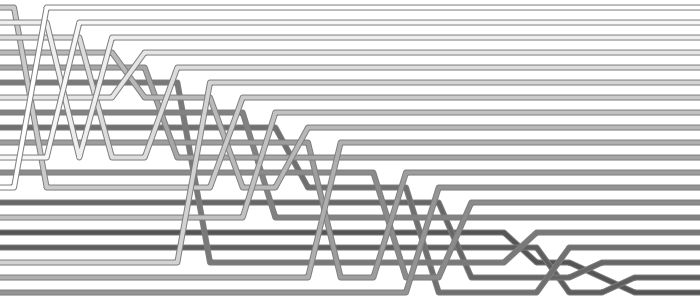
\includegraphics[width=\linewidth]{selection.png}

  \centerline{Algorithme A.}
\end{minipage}\hfill\begin{minipage}{.35\linewidth}
  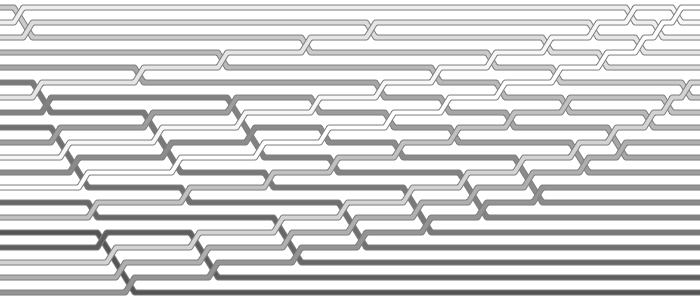
\includegraphics[width=\linewidth]{bubble.png}

  \centerline{Algorithme B.}
\end{minipage}\hfill\begin{minipage}{.35\linewidth}
  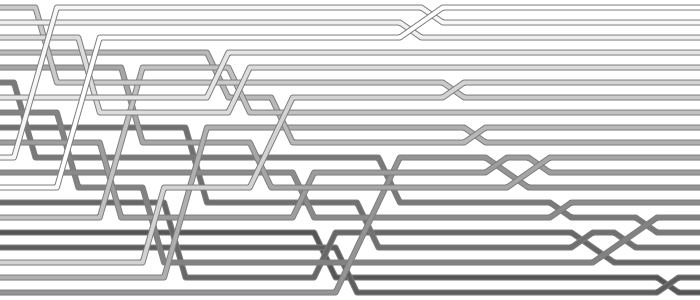
\includegraphics[width=\linewidth]{shell.png}

  \centerline{Algorithme C.}
\end{minipage}\hfill}~

%%%%%%%%%%%

\noindent\hfill\begin{minipage}{.35\linewidth}
  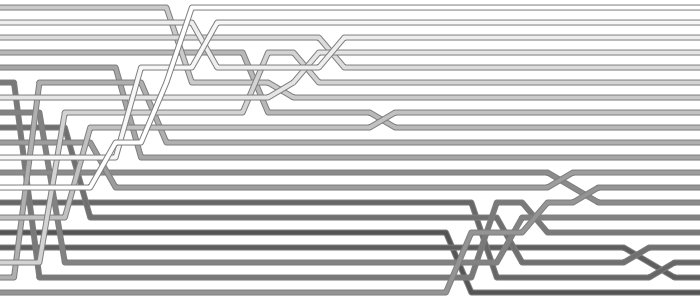
\includegraphics[width=\linewidth]{quick.png}

  \centerline{Algorithme D.}
\end{minipage}\hfill\begin{minipage}{.35\linewidth}
  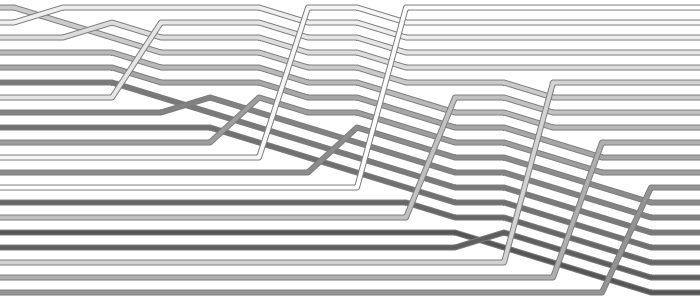
\includegraphics[width=\linewidth]{insertion.png}

  \centerline{Algorithme E.}
\end{minipage}\hfill~

\begin{Reponse}
  \textbf{Tri a bulle:} parcours successifs du tableau en comparant les voisins
  2 à 2. S'ils sont mal triés, on les inverse. Ce comportement a tendance à
  pousser les grosses valeurs vers la fin. On peut reconnaitre ce comportement
  dans l'algorithme B.

  \textbf{Tri par insertion:} invariant: ce qui est avant la frontière est
  trié. A chaque étape, je prend l'élément juste après la frontière, et je le
  met à sa place dans la partie déjà triée. On peut reconnaitre ce comportement
  dans l'algorithme E.

  \textbf{Tri par selection:} a chaque étape, je selectionne le minimum de la
  partie non triée et le pose à la frontière. On reconnait l'algorithme A.

  \textbf{Shell sort:} comme un bubble sort, mais on commence par trier avec un
  écartement supérieur à 1. Au lieu d'inverser des voisins, on inverse des
  cases à distance 3 puis 2 puis on fait un bubble standard, mais sur un
  tableau un peu prétrié. C'est l'algorithme C.

  \textbf{Quick sort:} c'est un algorithme récursif qui trie une partie du
  tableau puis l'autre (les parties ne sont pas forcément de taille
  identique). C'est l'algorithme D.
\end{Reponse}


\end{document}


%%% Local Variables:
%%% coding: utf-8
